\begin{figure}[t]
\eightpoint
\begin{Verbatim}[numbers = left]
float->float pipeline Main {
  add Source();  // code for Source not shown
  add AssignPictureType();
  add Output();  // code for Output not shown
}

int->int filter AssignPictureType(int width, 
        int height, 
        int numpictures) {
    int frameno;

    init {
        frameno = 0;
    }

    work pop (width*height*3) push 2 {
        push(frameno);
        for (int i = 0; i < width*height*3; i++) {
            pop();
        }

        int pushval;
        int framecount = frameno % 12;
        if (framecount == 0) {
            pushval = 1;
        } else if (framecount == 3 
                || framecount == 6 
                || framecount == 9) {
            pushval = 2;
        } else {
            pushval = 3;
        }

        if ((frameno == (numpictures-1)) 
            && (pushval == 3)) {
            pushval = 2;
        }

        push(pushval);
        frameno++;
    }
}
\end{Verbatim}

\caption{Example StreamIt program with AssignPictureType filter, used in MPEG Encoder.\protect\label{fig:apt-pipeline}}
\end{figure}

\section{The StreamIt Language}
\label{sec:streamit}

StreamIt is an architecture-independent language for high-performance
stream programming~\cite{thies-cc02}.  The compiler is publicly
available~\cite{streamitweb} and includes backends for multicore
architectures, clusters of workstations, and Tilera architectures.

The model of computation in StreamIt is grounded in (but not limited
to) synchronous dataflow~\cite{lee87}.  In this model, the programmer
implements independent actors, or {\it filters}, which translate data
items from input channels to output channels.  Filters are composed
into graphs that represent the overall computation.  The key property
of synchronous dataflow is that the number of items consumed and
produced during each execution of a filter is known at compile time,
allowing the compiler to perform static scheduling and optimization.

An example StreamIt program appears in Figure~\ref{fig:apt-pipeline}.
It is based on the AssignPictureType filter in the MPEG-2 encoder.
StreamIt filters contain three stages of execution.  The most
important is the {\it work} function, which represents the
steady-state execution step and is called repeatedly by the runtime
system.  Within the work function, a filter may {\it peek} at a given
element on the input tape, {\it pop} an item off the input tape, or
{\it push} an item to the output tape.  The total number of items
peeked, popped, and pushed are declared as part of the work function.
Note that if the peek rate exceeds the pop rate, it represents a
sliding window computation in which some input elements are accessed
across multiple invocations of the filter.

In addition to the work function, a filter may declare an {\it init}
function to initialize internal data structures, as well as a {\it
  prework} function (not given in Figure~\ref{fig:apt-pipeline}) to
perform specialized processing of data items prior to the steady
state.  The prework function is needed in cases where the initial
processing has a different input or output rate than the steady-state
processing.

A {\it schedule} gives a multiplicity for each filter in a stream
graph.  The multiplicity indicates how often a filter's {\it work} function
should be invoked (or {\it prework} function on the first iteration of the filter).  The
{\it steady-state schedule} can be calculated such that all filters
fire in the schedule, and the schedule can be repeated
indefinitely~\cite{lee87}.  Steady-state execution of the graph
entails repeating the steady-state schedule for as much input as is
expected.  Execution of the stream graph is conceptually wrapped in an
outer loop that continuously executes the steady-state schedule.  All
the multiplicities of the steady-state can be multiplied by the same
constant $c$, and the result will still be a valid steady-state.  We
call this process {\it increasing} the steady-state of the graph by
$c$.

Furthermore, an {\it initialization} schedule enables the steady-state
schedule in the presence of peeking filters.  An initialization
schedule is required if peeking is present in a graph to enable the
calculation and execution of a steady-state
schedule~\cite{karczmarek-lctes03}.  During application execution, the
{\it init} function is called once for each filter, then the
initialization schedule is executed once, followed by an infinite
repetition of the steady-state schedule.

As depicted in Figure~\ref{fig:structures}, StreamIt provides three
hierarchical primitives for composing filters into stream graphs.  A
{\it pipeline} represents a sequential composition of streams, in
which the output of one stream feeds into the input of the next.  A
{\it splitjoin} represents a parallel set of streams, which divulge
from a common {\it splitter} and converge to a common {\it joiner}.
The types of splitters and joiners are predefined by the StreamIt
language; they encompass duplication and weighted round-robin
behaviors.  Finally, a {\it feedbackloop} represents a cycle in the
stream graph.

\begin{figure}[t!]
\centering
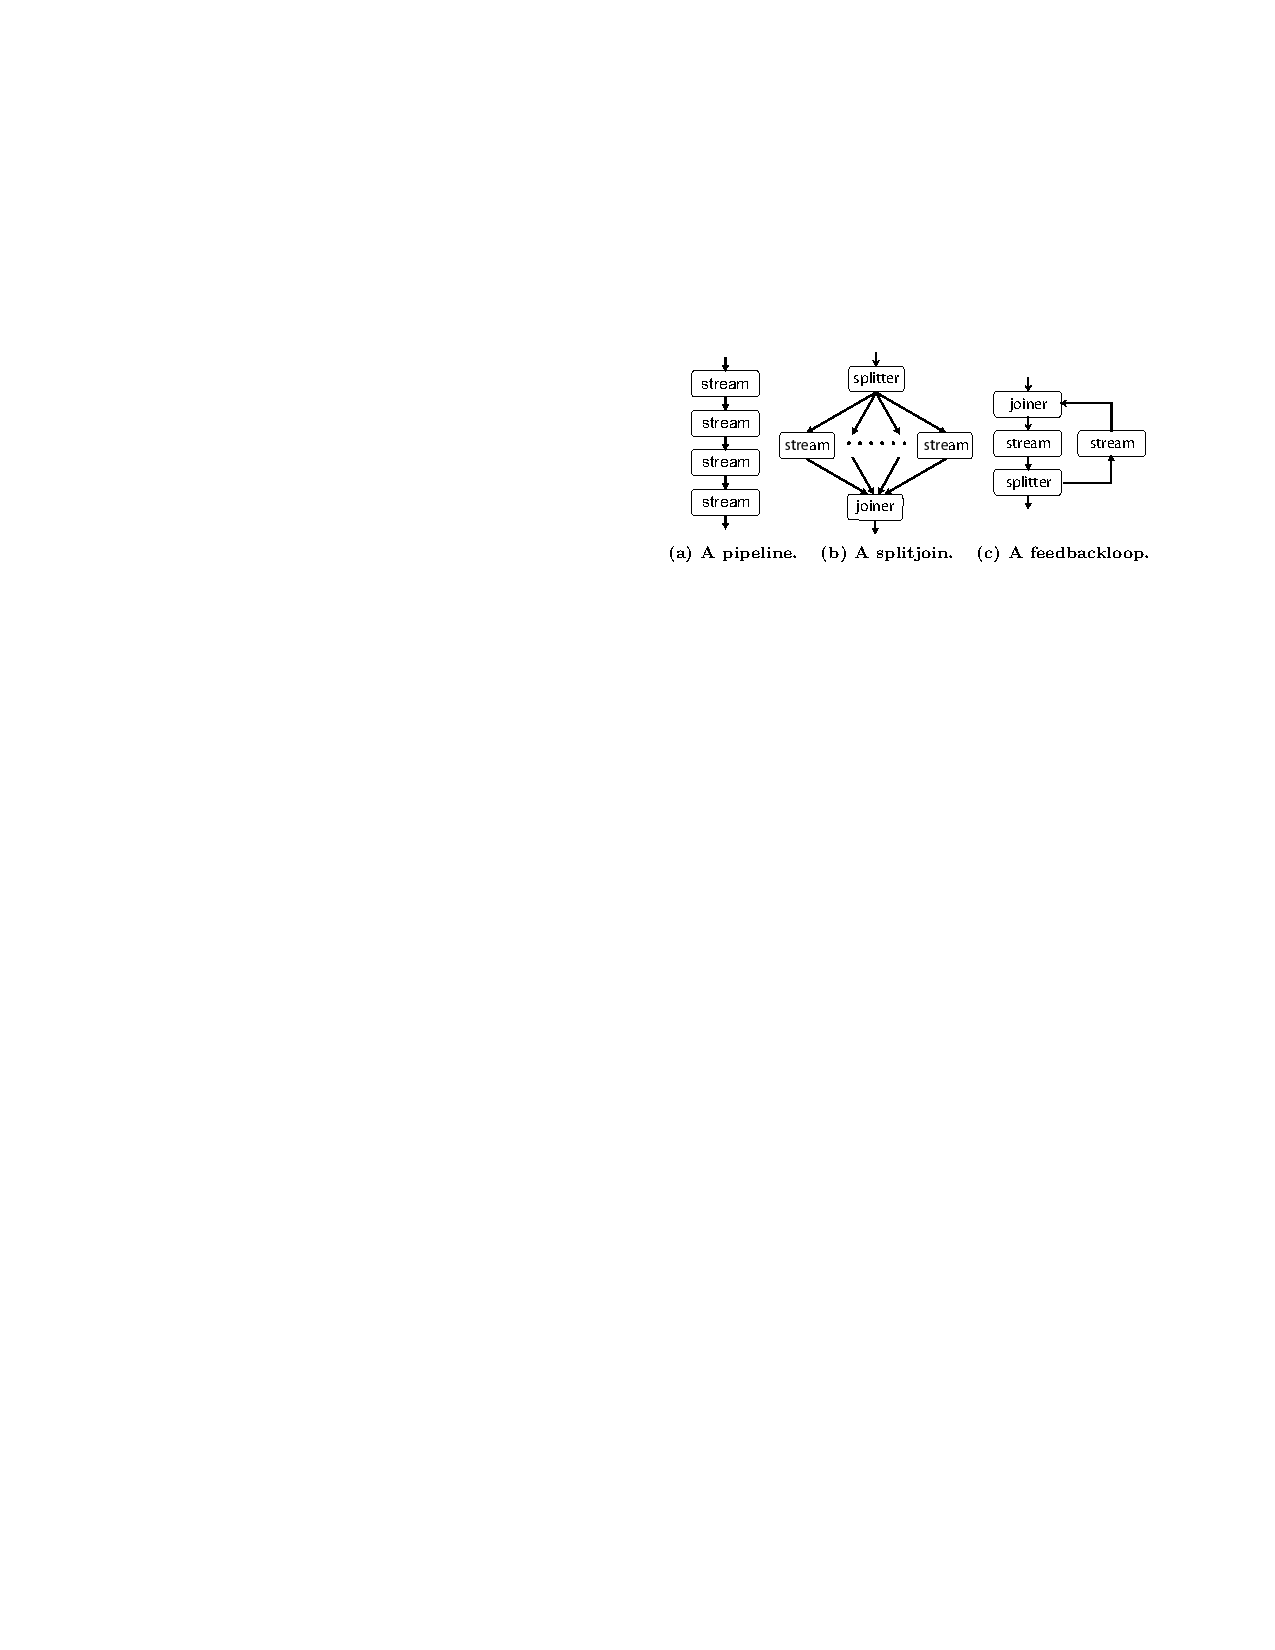
\includegraphics[width=3.3in]{stream-structures.pdf}
%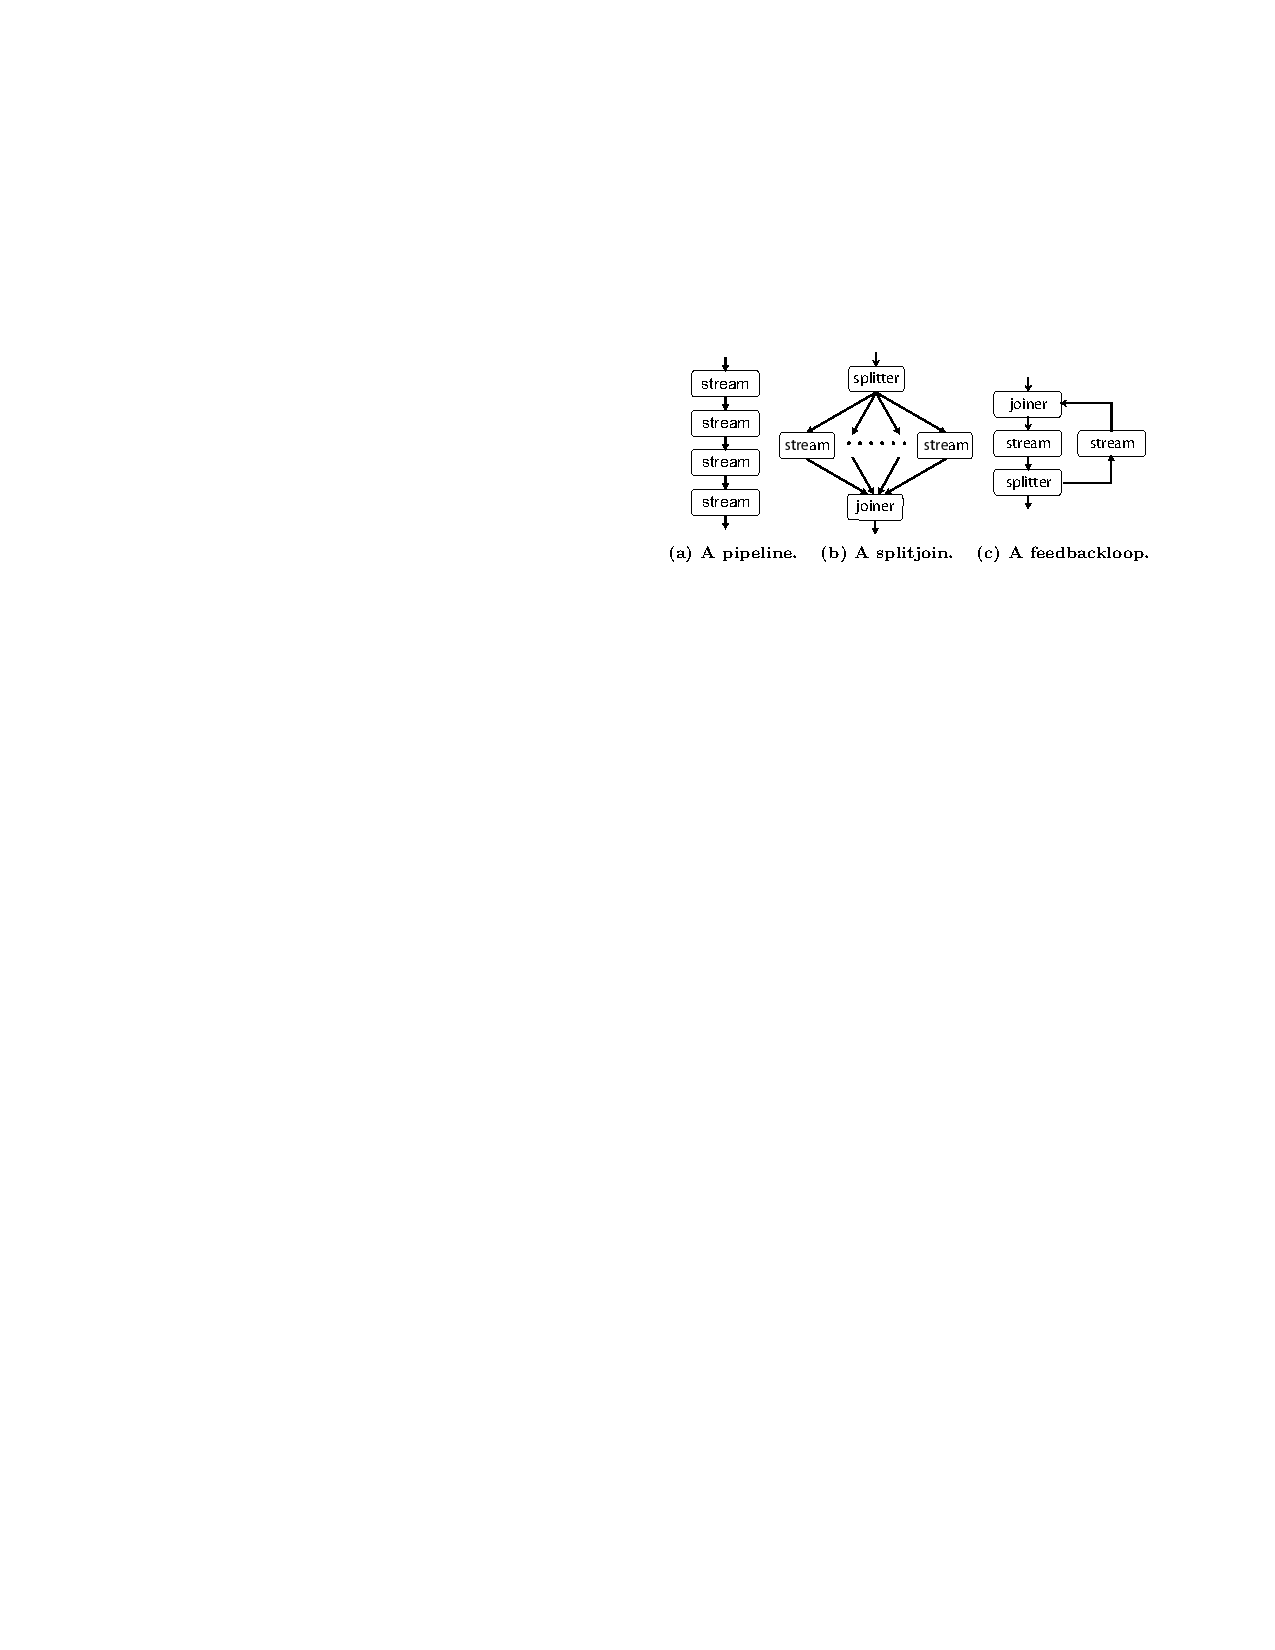
\psfig{file=stream-structures,width=\columnwidth}
\caption{Hierarchical stream structures supported by StreamIt.\protect\label{fig:structures}}
\end{figure}

The StreamIt compiler coarsens the granularity of a stream graph by
applying the {\it fusion} transformation which merges adjacent filters
into a single (large) filter (embedding the schedules of execution in
the merged filter)~\cite{streamit-asplos}.  The {\it fission}
transformation is employed to add data parallelism to a stream graph.
In fission, a single filter without state is duplicated a certain
number of ways and placed in a splitjion construct.  Input items to
the original filter are distributed among the duplicates, termed {\it
  fission products}.  In \S\ref{sec:fission}, we describe how to
extend the fundamental fission transformation to parallelize induction
variable state.
